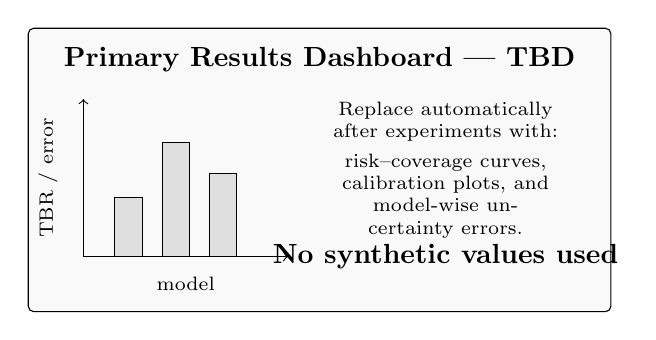
\begin{tikzpicture}[font=\scriptsize]
\draw[rounded corners=2pt, fill=gray!5] (0,0) rectangle (7.4,3.6);
\node[font=\bfseries] at (3.7,3.2) {Primary Results Dashboard --- TBD};
\draw[->] (0.7,0.7) -- (0.7,2.7); \draw[->] (0.7,0.7) -- (3.3,0.7);
\node[rotate=90] at (0.25,1.7) {TBR / error}; \node at (2.0,0.35) {model};
\draw[fill=gray!25] (1.1,0.7) rectangle (1.45,1.45); \draw[fill=gray!25] (1.7,0.7) rectangle (2.05,2.15); \draw[fill=gray!25] (2.3,0.7) rectangle (2.65,1.75);
\node[align=center, text width=32mm] at (5.3,1.8) {Replace automatically after experiments with:\\[1mm]risk--coverage curves,\\calibration plots, and\\model-wise uncertainty errors.};
\node[font=\bfseries] at (5.3,0.7) {No synthetic values used};
\end{tikzpicture}
